\chapter{Sequential Consistency Logic}
\label{ch:seqcon}

  \subsection{Summary}

  The subsequent development of this thesis is conceptually based on
  intuitionistic epistemic logic that appeared in the Master's thesis
  of the author.
  We contain the relevant motivations, definitions and results in this chapter.
  However, we omit proofs that
  can be found in the Master's thesis.
  We add the finite model property of sequential consistency logic
  with the full details because that result is not found in the Master's thesis.

  In this chapter, we give a logic called intuitionistic epistemic logic.
  The logic has epistemic modality $K_a$ in addition to ordinary logical connectives
  $(\wedge, \vee, \supset, \bot)$ of propositional logic.
  We explain the meaning of the new modality $K_a$ informally, by extending
  the Brouwer--Heyting--Kolmogorov interpretation (BHK-interpretation) of logical
  connectives, which dates back to 1930's
  (Heyting~\cite{heyting1930formalen, heyting1931intuitionistische}
  are cited by Troelstra et al.~\cite{troelstra1988constructivism}).

  Intuitionistic logic is originally a formalisation of a single mathematician whose
  knowledge
  increases over time.  The logic \iec\, formalises multiple agents who communicate
  asynchronously and whose knowledge increases over time.
  The logic \iec\, has a simple language:
  it has epistemic modality but no temporal modality
  so that it is simpler than many previous logics for communication.
  We do not need temporal modality because
  we regard time as
  the partial order in the semantics of intuitionistic epistemic logic.
  Before defining the deduction system, we first extend the informal intuitionistic
  reading of logical connectives.
  Precisely,
  we extend Brouwer--Heyting--Kolmogorov interpretation of logical connectives
  by adding one clause reagarding the additional epistemic modality~$K_a$.
  After stating the informal meaning for the modality,
  we define a deduction system and a Kripke semantics meeting this intuition.
  Soundness, strong completeness, finite
  model property, disjunction property and decidability are
  shown.
  We also investigate the relationship between \iec\,and classilcal modal logic with multple
  S4 modalities.

  On top of the logic \iec, we give an axiom type that characterises
  sequential consistency for shared memory.
  The advantage of intuitionistic logic over classical logic is shown
  in an example where a set of axioms characterises
  sequential consistency on shared memory.
  The axioms for sequential consistency are
  meaningless in classical logic while
  meaningful in intuitionistic logic.
  The axioms are similar to
  the axiom type for prelinerilty.
  This similarity reflects the analogy
  between sequential consistency for shared memory scheduling
  and linearity for Kripke frames: both require antisymmetry on schedules or models.

  Finally, under sequential consistency, we give soundness and completeness between
  a set of logical formulae called waitfree assertions and a set of models called
  schedule models.
  It has been found that it is undecidable whether a task is waitfreely solvable or not.
  We show that when we only view the communication requirements of tasks,
  it is decidable whether the communication is waitfreely attainable or not.

  There are at least two different ways of reasoning about knowledge.
  In one view of knowledge using Kripke semantics,
  which classical epistemic logic employs,
  knowledge is defined as proposition valid in all possible worlds
  that is possible to an agent.
  On the other hand, knowledge can be seen as something agents can send and receive.
  We unify these two notions of knowledge into the semantics of the logic we present.
  We define the semantics formally in the style of Kripke semantics.
  At the same time,
  an extension to BHK-interpretation reveals that asynchronous
  communication is implicit in the formal definition.

  \subsection{The Reason for Another Logic}

    \paragraph{Motivation: reasoning about concurrent systems}
    We give a formal deduction system for reasoning about
    asynchronous communication.
    The motivation for doing it is
    the fact that creating a concurrently
    working system with asynchronous communication
    and especially testing and debugging it is
    notoriously difficult
    because of nondeterministic scheduling.
    When the cost of testing and debugging is high,
    it is reasonable to
    spend more cost on ensuring correctness of the system
    at earlier stages like designing phase or implementation phase, not testing and debugging.
    In order to ensure correctness at an earlier stage,
    it is crucially important to reason about the system correctly because
    at such an early stage, knowledge about the system can only be obtained by reasoning,
    not by testing.

    \paragraph{Method: giving a formal deduction system}
    A formal deduction system mathematically defines
    available form of reasoning.
    In order to define reasoning mathematically,
    a formal deduction system uses languages defined mathematically.
    The main advantage of the reasoning on a formal deduction system over
    reasoning in a natural language
    is the former is independent of most implicit assumptions
    on which the latter is dependent so that
    the validity of the former formal reasoning can be checked more rigorously
    than the latter informal reasoning.

    We seek to have a formal
    deduction system as simple and learnable as possible to reason about asynchronous
    communication.
    We choose to give an epistemic logic, i.e., a logic with an operator expressing an agent's
    knowledge because mentioning agents' knowledge appeals to
    human intuition.
    For example, as Halpern and Zuck~\cite{halpern1992little}
    point out, Bochmann and Gecsei's paper~\cite{bochmann} written in 1977 already uses
    the notion of knowledge when reasoning about protocols:
    \begin{quotation}
     \noindent
     Verification \ldots will correspond
     \ldots to finding out whether and in
     which circumstances the sender \ldots
     can ``know'' that all data \ldots have been delivered correctly%
     \footnote{The dots \ldots and a period by the author.}.
    \end{quotation}

  \subsection{Intuitionistic Epistemic Logic}

  The main contribution of this thesis is giving definition of
  intuitionistic epistemic logic (\iec\, for short) and investigating it.

    \paragraph{Original intuitionistic meaning of knowledge}
    Agents in asynchronous systems can
    obtain knowledge about other agents only by receiving some constructions from them,
    not by waiting for a fixed length of time.
    This specific style of knowledge, where
    obtaining knowledge requires obtaining physical constructions,
    is the same as the style of knowledge of intuitionistic, constructive reasoners.
    That is the reason why we deliberately choose intuitionistic not classical meanings for
    the basic logical connectives, especially $\supset$ and $\vee$, although classical logic
    is more popularly used among computer scientists and mathematicians.
    The abstract Kripke model for asynchronous communication
    can be seen as a description of agents passing around constructions that ensure
    propositions.

    We extend the language of intuitionistic propositional logic with a unary operator $K_a$,
    whose meaning can be expressed as:
    a proof of $K_a\varphi$ is a construction that witnesses agent~$a$'s
    acknowledgement of a proof of $\varphi$ and also contains the acknowledged
    proof.  This formulation of knowledge is original.
    This meaning is different from that of classical epistemic logic where
    the meaning of $K_a$ can be expressed as:
    $K_a\varphi$ is valid if and only if $\varphi$ is valid in all possible worlds
    that agent~$a$ thinks possible.

    One advantage of our meaning of $K_a$ over that of classical meaning is that
    it can express communication without the help of another modality.
    Namely, in our meaning,
    a proof of $K_bK_a P$ is a construction that is passed from agent $a$ to agent
    $b$.
    On the other hand, in classical meaning, the same formula expresses nothing about
    communication:
    $K_b K_a P$ is valid when $P$ is valid in all possible worlds that agent~$b$ in any
    possible world that agent~$a$ thinks possible thinks possible.

    Intuitionistic logic can be seen as a logic describing an agent whose knowledge increases over
    time.
    The logic \iec\,  can be seen as a logic describing multiple agents
    that asynchronously communicate with each other and increase their knowledge.
    Although \iec\, deals with communication, the logic has only epistemic modalities so that it
    has simpler syntax than many other logics for communication.

    We give a deduction system and show
    soundness (\thref{soundness}),
    disjunction property (\thref{disjunction-property}),
    strong completeness
    (\thref{strong-completeness}), finite model property
    (\thref{thm:fmp}) and decidability (\thref{decidability}).

  \subsection{Application to Waitfree Communication}

    \paragraph{Sequential consistency}
    The topological characterisation by Herlihy and Shavit~\cite{herlihy1999topological}
    implicitly assumes sequential consistency~\cite{lamport1979make} of shared memory.
    This motivated us to characterise sequential consistency with the axiom type
    $(K_\memory \varphi\supset K_\memory \psi)\vee (K_\memory
       \psi\supset K_\memory \varphi)$
       in the logic \iec\, for asynchronous computation.
       Technically, we defined a class of models called sequential models
       and proved soundness
       (\thref{sc-sound}) and completeness
       (\thref{sc-comp}) of the axiom type with respect to the sequential models.

    \paragraph{Waitfree communication}
    A waitfree protocol over shared memory~\cite{herlihy1991wait}
    assigns a program to each process so that no process waits for another process.
    Some tasks can be solved by a~well-chosen waitfree protocol while the others cannot.

    For example,
    it is waitfreely impossible for both of two processes to attain the input value of the other
    process.
    On the other hand, it is waitfreely possible for
    either one of two processes to attain the input value of the other process.
    A waitfree protocol that solves this task is:
    \begin{itemize}
     \item process $a$ tells the memory $\memory$ that $\varphi$ holds, and then $\memory$ replies back to $a$,
     \item process $b$ tells the memory $\memory$ that $\psi$    holds, and then $\memory$ replies back to $b$.
    \end{itemize}
    After this protocol finishes,
    either $\varphi$ has been communicated from~$a$ to~$b$
    or $\psi$ has
    been communicated from~$b$ to~$a$.

    In the
    logic \iec, this fact is represented by a judgement $K_aK_\memory{}K_a\varphi,
    K_bK_\memory{}K_b\psi\vdashsc K_aK_b\psi\vee K_bK_a\varphi$,
    which is deducible in \iec\, with
    sequential consistency axioms~(Figure~\ref{hoge}).

    Herlihy and Shavit~\cite{herlihy1999topological} characterised waitfree computation using
    simplicial topology.
    Using their characterisation,
    Gafni and Koutsoupias~\cite{gafni1999three}
    showed that it is undecidable whether a task is waitfreely solvable
    or not.
    When tasks are restricted to communication defined by
    a class of logical formulae that we call waitfree assertions,
    we can characterise waitfreely available communication logically (\thref{sc-comp})
    and
    it is decidable whether a task is waitfreely solvable or not (\thref{wf-dec}).

  \subsection{Formulae}

  We fix a countably infinite set of propositional symbols
  $\pvar$ and a finite set of agents $A$.
  Let $P, Q, \ldots$ run over the propositional symbols.

  \begin{definition}
   \label{formula}
   We define a \iec-formula\index{formula!\iec-formula} $\varphi$ by the BNF:
   \[
   \varphi ::= \bot\mid P\mid
   (K_a\varphi)\mid(\varphi\vee\varphi)\mid(\varphi\land\varphi)\mid
   (\varphi\supset\varphi)
   \]
   where $a\in A$ stands for an agent.
  \end{definition}
  We sometimes omit the parenthesis when no confusion occurs. We use $=$ for syntactic
  equality of formulae.
  \noindent The unary operators connect more strongly than the binary operators.
  We sometimes omit the parentheses when no confusion occurs. We use $=$ for syntactic
  equality of formulae.  The notation $(\neg \varphi)$ stands for $(\varphi\supset \bot)$.
  The notation~$\top$ stands for $(\bot\supset\bot)$.
  For a sequence of \iec-formulae $\Gamma = (\varphi_i)_{i\in I}$ or a set of \iec-formulae~$\Gamma$,
  the notation $K_a \Gamma$ stands for the sequence $(K_a \varphi_i)_{i\in I}$ or the set
  $\{K_a\varphi\mid \varphi\in \Gamma\}$ respectively.

  \subsection{Informal Explanation by BHK-Interpretation}
  \label{bhk}

  Intuitionistic meanings for logical connectives
  can be presented as
  following sentences called BHK-interpretation\footnote{
  Taken from Troelstra and van Dalen's textbook~\cite[Ch.~1]{troelstra1988constructivism}:
  author made notational modification of logical formulae and omission of
  quantifiers $\forall$ and $\exists$.
  }:
  \begin{quotation}
   \noindent
   \begin{description}
    \item[(H1)] A proof of $\varphi\land \psi$ is given by presenting a proof of $\varphi$
	 and a proof of $\psi$.
    \item[(H2)] A proof of $\varphi\vee\psi$ is given by presenting either a proof of
	 $\varphi$ or a proof of $\psi$ (plus the stipulation that we want to regard
	 the proof presented as evidence for $\varphi\vee\psi$\footnote{In fact, the
	 author considers this as not enough. A proof $\varphi\vee\varphi$ must contain
	 the choice of the left $\varphi$ or the right $\varphi$.  This
	 allows us to encode a Boolean value as a proof of $(\top\lor\top)$}).
    \item[(H3)] A proof of $\varphi\supset\psi$ is a construction which permits us to
	 transform any proof of $\varphi$ into a proof of $\psi$.
    \item[(H4)] Absurdity $\bot$ (contradiction) has no proof; a proof of $\neg \varphi$ is a
	 construction which transforms any hypothetical proof of $\varphi$ into a proof
	 of a contradiction.
   \end{description}
  \end{quotation}
  In this paper, we consider extending BHK-interpretation with another stipulation for
  epistemic modality:
  \begin{description}
   \item[(HK)] A proof of $K_a\varphi$ is a construction that witnesses agent~$a$'s
	acknowledgement of a proof of $\varphi$ and also contains the acknowledged
	proof.
  \end{description}
  We choose to regard knowledge as acknowledgement of proofs so that the modality $K_a$ informally
  describes knowledge of agent~$a$.
  The formalisation of knowledge is different from that in classical epistemic logic, where
  knowledge is described as a limitation on the ability to distinguish possible worlds.

  \subsection{Deduction System}

  \begin{figure*}
   \begin{center}
    \AxiomC{}
    \LeftLabel{(ax)}
    \UnaryInfC{$\varphi \vdash \varphi$}
    \DisplayProof
    \hfill
    \AxiomC{$\Gamma\vdash\varphi$}
    \LeftLabel{(w)}
    \UnaryInfC{$\psi,\,\Gamma\vdash\varphi$}
    \DisplayProof
    \hfill
    \AxiomC{$ \varphi,\,\varphi,\,\Gamma\vdash\varphi'$}
    \LeftLabel{(c)}
    \UnaryInfC{$\varphi,\,\Gamma\vdash\varphi'$}
    \DisplayProof
    \hfill
    \AxiomC{$\Gamma, \varphi,\psi,\, \Gamma'\vdash\varphi'$}
    \LeftLabel{(e)}
    \UnaryInfC{$\Gamma,\,\psi,\varphi,\,\Gamma'\vdash\varphi'$}
    \DisplayProof
    \vskip 5mm
    \AxiomC{$\Gamma\vdash \varphi\land\psi$}
    \LeftLabel{($\wedge$-E$_0$)}
    \UnaryInfC{$\Gamma\vdash \varphi$}
    \DisplayProof
    \hfill
    \AxiomC{$\Gamma\vdash\varphi$}
    \AxiomC{$\Gamma'\vdash\psi$}
    \LeftLabel{($\wedge$-I)}
    \BinaryInfC{$\Gamma,\Gamma'\vdash \varphi\land\psi$}
    \DisplayProof
    \hfill
    \AxiomC{$\Gamma\vdash \varphi\land\psi$}
    \LeftLabel{($\wedge$-E$_1$)}
    \UnaryInfC{$\Gamma\vdash \psi$}
    \DisplayProof
    \vskip 5mm
    \AxiomC{$\Gamma\vdash \varphi$}
    \LeftLabel{($\vee$-I$_0$)}
    \UnaryInfC{$\Gamma\vdash \varphi\vee\psi$}
    \DisplayProof
    \hfill
    \AxiomC{$\Gamma\vdash \varphi$}
    \LeftLabel{($\vee$-I$_1$)}
    \UnaryInfC{$\Gamma\vdash \psi\vee\varphi$}
    \DisplayProof
    \vskip 5mm
    \AxiomC{$\Gamma\vdash \psi_0\vee\psi_1$}
    \AxiomC{$\Gamma,\,\psi_0\vdash \varphi$}
    \AxiomC{$\Gamma,\,\psi_1\vdash \varphi$}
    \LeftLabel{($\vee$-E)}
    \TrinaryInfC{$\Gamma\vdash \varphi$}
    \DisplayProof
    \vskip 5mm
    \AxiomC{$\varphi,\,\Gamma\vdash\psi$}
    \LeftLabel{($\supset$-I)}
    \UnaryInfC{$\Gamma\vdash \varphi\supset\psi$}
    \DisplayProof
    \hfill
    \AxiomC{$\Gamma\vdash\psi_0\supset\psi_1$}
    \AxiomC{$\Gamma\vdash \psi_0$}
    \LeftLabel{($\supset$-E)}
    \BinaryInfC{$\Gamma\vdash \psi_1$}
    \DisplayProof
    \hfill
    \AxiomC{$\Gamma\vdash\bot$}
    \LeftLabel{($\bot$-E)}
    \UnaryInfC{$\Gamma\vdash\varphi$}
    \DisplayProof
    \hfill
    \AxiomC{$\Gamma\vdash K_a\varphi$}
    \LeftLabel{(T)}
    \UnaryInfC{$\Gamma\vdash \varphi$}
    \DisplayProof
    \vskip 5mm
    \AxiomC{$\Gamma \vdash K_a\varphi$}
    \LeftLabel{(ispec)}
    \UnaryInfC{$\Gamma\vdash K_a K_a \varphi$}
    \DisplayProof
    \hfill
    \AxiomC{$\Gamma\vdash\varphi$}
    \LeftLabel{(nec)}
    \UnaryInfC{$K_a\Gamma\vdash K_a\varphi$}
    \DisplayProof
    \hfill
    \AxiomC{$\Gamma\vdash K_a(\varphi\vee\psi)$}
    \LeftLabel{($\vee K$)}
    \UnaryInfC{$\Gamma\vdash K_a \varphi\vee K_a\psi$}
    \DisplayProof
   \end{center}
   \caption[Deduction rules of \iec.]
   {Deduction rules of \iec.  (ax) stands for axiom, (w) for weakening, (c) for
   contraction, (e) for exchange, (ispec) for introspection and (nec) for necessitation.
   ($\diamondsuit$-I) denotes the introduction rule for connective~$\diamondsuit$.
   ($\diamondsuit$-E) denotes the elimination rule for connective~$\diamondsuit$.}
   \label{fig}
  \end{figure*}

  We give a proof system of \iec\, in the natural deduction~\citep{gentzen, prawitz1971ideas}.
  All the rules that do not mention modalities are common with
  intuitionistic propositional logic while the other rules are added
  to define the meaning of the $K_a$ modality.
  \begin{definition}
   We define the proof system of \iec\, by Figure~\ref{fig}.
   The system is presented in the form of usual schemata.
   A proof diagram is a finite tree of deduction rules with one bottom node with the
   following property: when a node has a judgement
   above the line, there is a node immediately above it and the above node
   has the same judgement below the line.
  \end{definition}

    \paragraph{Rationales for the rules on modalities}

    While the rules (T), (ispec) and (nec) are admissible in classical S5 epistemic logic,
    we have an additional rule ($\vee K$) which needs explanation.
    In this paragraph, we are going to give a rationale for the rule ($\vee K$) with the help
    of BHK-interpretation given in Subsection~\ref{bhk}.
    A proof for the premise of the rule ($\vee K$) is a construction that witnesses agent~$a$'s
    acknowledgement of a proof of $\varphi\vee\psi$.
    Since a proof of $\varphi\vee\psi$ is either a proof of $\varphi$ or a proof of $\psi$,
    agent~$a$'s acknowledge of a proof of $\varphi\vee\psi$ implies either agent~$a$'s
    acknowledgement of a proof of $\varphi$ or agent~$a$'s acknowledgement of a proof of $\psi$.

    Also,
    we are informally
    assuming logical omniscience of the agents by rule (nec),
    that is, we assume agents have complete
    command on intuitionistic epistemic logic so that they acknowledge every \iec-formulae
    deducible from the set of \iec-formulae they acknowledge.

    \paragraph{Notational conventions}
    For a set of \iec-formulae~$\Gamma$ and an~\iec-formula~$\varphi$, $\Gamma\vdash
    \varphi$ denotes a~relation where
    there is such a~finite sequence~$\Gamma_0$ that
    $\Gamma_0\vdash
    \varphi$ is deducible and that $\Gamma_0$ is contained in $\Gamma$.

  \subsection{Semantics}
  We define validity of a~\iec-formula on a~state in a~model.
  A~model is a~Kripke model for propositional intuitionistic logic
  equipped with an additional
  mapping $f_a: W\rightarrow W$ for each agent $a\in A$ where $W$ is the
  set of possible states.
  Informally\footnote{This account is informal in that we do not attempt to
  define the terms ``view'' and ``current state.''},
  the function $f_a$ represents the view of agent
  $a$.
  When the current state is $w\in W$\kern -2pt, agent $a$ sees that the current state is
  $f_a(w)\in W$, in other words, agent $a$ knows everything valid in $f_a(w)$.
  As a special consequence, agent $a$ knows that agent $b$ sees that the current state
  is
  $f_b(f_a(w))\in W$\kern -2pt.

  \newcommand{\model}[1]{\tuple{W#1, \preceq#1, (f_a#1)_{a\in A}, \rho#1}}
  \begin{definition}
   \label{model}
   A model\index{model} $\tuple{W,\preceq, (f_a)_{a\in A}, \rho}$ is a tuple with following properties:
   \begin{enumerate}
    \item $\tuple{W,\preceq}$ is a partial order,
    \item $f_a\colon W\rightarrow W$ is a~function satisfying
	  \begin{enumerate}
	   \item (decreasing) $f_a(w) \preceq w$,
	   \item (idempotency) $f_a(f_a(w)) = f_a(w)$, and
	   \item (monotonicity) $w\preceq v$ implies $f_a(w)\preceq f_a(v)$
	  \end{enumerate}
	  for all $v,w\in W$, and
    \item $\rho\colon \pvar\rightarrow \powerset W$ is a function such that each $\rho(P)$ is
	  upward-closed with respect to $\preceq$, i.e., $w'\succeq w\in\rho(P)$ implies
	  $w'\in\rho(P)$.
   \end{enumerate}
  \end{definition}
  \noindent With the informal account in mind, the conditions on $f_a$ have rationales:
  decreasing condition says an agent~$a$ recognises only truth,
  idempotency says an agent $a$ recognises that
       $a$ recognises something whenever the agent~$a$ recognises that thing,
       and monotonicity says an agent~$a$ does not forget things recognised.
       Differently from classical epistemic logic,
       there is no distinction between global states and local states.

       The valuation~$\rho$ for propositional variables in $\pvar$ is extended into validity
       relation~$\models$ for all \iec-formulae in $\fml$.
       \begin{definition}
	We define the satisfaction relation\index{satisfaction} $\models$ of a~model
	$\tuple{W,\preceq,(f_a)_{a\in A},\rho}$, a~state~$w\in W$ of the model and an
	\iec-formula~$\varphi$.
	Let us fix a model $M=\tuple{W,\preceq,(f_a)_{a\in A},\rho}$.
	\newcommand{\m}{M}
	The definition of $M,w\models\varphi$ is inductive on the structure of $\varphi$.
	\begin{description}
	 \item[(Case $\varphi=\bot$)] $\m, w\models \bot$ never holds.
	 \item[(Case $\varphi= P$)] $\m, w\models P$ if and only if
	      $w \in
	      \rho(P)$.
	 \item[(Case $\varphi = K_a \psi$)]
	      $\m, w\models K_a \psi$ if and only if
	      $\m, f_a(w)\models \psi$.
	 \item[(Case $\varphi = \psi_0\land\psi_1$)]
	      $\m, w\models \psi_0\land\psi_1$ if and only if both
	      $\m, w\models \psi_0$ and $\m,w\models \psi_1$ hold.
	 \item[(Case $\varphi = \psi_0\vee\psi_1$)]
	      $\m, w\models \psi_0\vee\psi_1$ if and only if at least
	      one of
	      $\m, w\models \psi_0$ or $\m,w\models \psi_1$ holds.
	 \item[(Case $\varphi = \psi_0\supset \psi_1$)]
	      $\m, w\models \psi_0\supset\psi_1$ if and only if
	      for any $w'\in W$ with $w'\succeq w$, the satisfaction $M,w'\models \psi_0$ implies
	      the satisfaction $M, w'\models
	      \psi_1$.
	\end{description}
       \end{definition}

       Next, we show that the monotonicity condition on the valuation~$\rho$ of
       propositional variables is preserved by the extension
       to satisfaction~$\models$ of \iec-formulae. Informally, this
       proposition
       reveals the limitation of the logic \iec:
       it can only deal with propositions whose satisfaction is preserved by progress with respect to
       the partial order $\preceq$.
       \begin{proposition}[Kripke monotonicity]
	\label{kripke}
	$M,w\models \varphi$ and $w\preceq v$ imply
	$M,v\models \varphi$.
       \end{proposition}
       \begin{proof}
	Straightforward using the monotonicity of $f_a$.
       \end{proof}

    \paragraph{Semantics of judgements}

    We introduce some notations which look similar to the judgements appearing in the
    deduction
    system.
    Being aware of the different definitions of $\vdash$ and $\models$, we are going to
    compare the two relations $\vdash$ and $\models$ in the next subsections.

    \begin{notation}
     For a~model~$M$ and a~state~$w$ of the model,
     we write $M,w\models \Gamma$ when the validity
     $M,w\models\varphi$ holds for any \iec-formula $\varphi$ in $\Gamma$.
    \end{notation}

    \begin{notation}
     $\Gamma\models\varphi$ stands for the relation of \iec-formula
     sequences $\Gamma$ and an \iec-formula
     $\varphi$ that holds if and only if for any model $M$
     and $w\in M$, $M,w\models \Gamma$ implies
     $M,w\models \varphi$.
    \end{notation}

    \begin{definition}
     $\Gamma\models\varphi$ stands for the relation of a set of \iec-formulae
     $\Gamma$ and an \iec-formula~$\varphi$ where $M,w\models \Gamma$ implies
     $M,w\models \varphi$ for any model~$M$
     and a~state~$w\in M$.
    \end{definition}
    For a~sequence of \iec-formulae $\Gamma$, we let $u(\Gamma)$ denote the set of \iec-formulae
    appearing in $\Gamma$.  We abbreviate $u(\Gamma)\models\varphi$ into
    $\Gamma\models\varphi$. We will write $\Gamma$ instead of $u(\Gamma)$ for the
    sake of brevity.

    \begin{definition}
     A set of \iec-formulae $\Gamma$ is consistent if and only if $\Gamma\not\models \bot$.
    \end{definition}

  \subsection{Soundness}

  A deduction system is called sound when existence of a proof of
  a sequent implies the corresponding semantic implication.
  Soundness is the most important feature of a formal deductive system because the
  main reason for using a formal deductive system is it ensures correct reasoning.
  We regard the defined semantics as a standard for correct reasoning and show that the
  deduction systems of \iec\, meets that standard.
  Soundness ensures an \iec-formula provable in \iec\, is valid in any state of any model.
  At the same time, we show a stronger notion:
  an \iec-formula provable under a set of assumptions is always valid whenever the assumptions are
  valid.

  \begin{proposition}[Soundness]
   \label{soundness}
   $\Gamma\vdash\varphi$ implies $\Gamma\models\varphi$.
  \end{proposition}
  Proof found in the author's Master's thesis.

  \subsection{Disjunction Property}

  Troelstra and van Dalen's
  textbook~\cite[3.5]{troelstra1988constructivism} says
  disjunction property is the test for constrictive logics.
  \fix{really they say so?}

   \begin{proposition}[Disjunction property]
    \label{disjunction-property}
    If $\vdash\varphi\vee\psi$ holds, either $\vdash\varphi$ or $\vdash\psi$ holds.
   \end{proposition}
   Proof to be found in the author's Master's thesis.

  \subsection{Strong Completeness and Finite Model Property}

  In this subsection, we show strong completeness and finite model property.
  Since both proofs contain model construction,
  most parts of both proofs can be written in the same propositions.
  This utilisation of similarity of finite model property and strong completeness
  is originally the idea of
  Sato~\cite{sato13study}.

  \fix{remove '}
  \begin{definition}
   We define $f'_a$ as:
   \[
   f'_a(\Gamma) = g_a(\Gamma) \cup K_ag_a(\Gamma).
   \]
  \end{definition}

  For some pages, we argue about a
  set of \iec-formula $\Omega$. Later, when we show
  strong completeness, we take $\Omega$ to be the whole set of well formed \iec-formulae.  Also,
  when we show finite model property, we take $\Omega$ to be the set of the subformulae of a
  certain \iec-formula.  This model construction is inspired by
  Sato's paper~\cite{sato13study}
  and Troelstra and van Dalen's textbook~\cite{troelstra1988constructivism}.
  However, the notion of $f'$-subformula-closed sets is new and original.

  \begin{definition}
   \label{saturated-set}
   For a set of formulae $\Omega$,
   a set of \iec-formulae $\Gamma\subseteq\Omega$ is $\Omega$-saturated%
   \index{saturated!$\Omega$-saturated} if and only if
   \begin{enumerate}
    \item $\Gamma$ is $\Omega$-deductively closed, i.e., $\Gamma\vdash\varphi\in
	  \Omega\Rightarrow
	  \varphi\in\Gamma$,
    \item $\Gamma\vdash\varphi\vee\psi \Rightarrow \Gamma\vdash\varphi$ or $\Gamma\vdash\psi$
	  if $\varphi,\psi\in\Omega$,
    \item $\Gamma\not\vdash\bot$.
   \end{enumerate}
  \end{definition}

  \begin{definition}
   A hereditary $f'$-subformula-closed set $\Gamma$ is coinductively defined as:
   $\Gamma$ is a hereditary $f'$-subformula-closed set if and only
   if $f'_a(\Gamma)$ is hereditary $f'$-closed, $\Gamma$ is closed for taking subformulae and
   $f'_a(\Gamma)\subseteq \Gamma$.
  \end{definition}

  \begin{definition}
   We define $s_a(\varphi)$ inductively on $\varphi$:
   \[
   s_a(\varphi) = \begin{cases}
		   s_a(K_a\psi) & \text{(if $\varphi = K_aK_a\psi$)},\\
		   \varphi & \text{(otherwise)}.
		  \end{cases}
   \]
  \end{definition}
  \noindent The function $s_a$ replaces every $K_aK_a$ with $K_a$ repeatedly so that there are no
  $K_aK_a$ occurrences left.

  \fix{is this lemma necessary?}
  \begin{proposition}
   \label{fpreserve}
   For a hereditary $f'$-subformula-closed set $\Omega$,
   if $\Gamma$ is an $\Omega$-saturated set,
   $f_a(\Gamma)$ is an $f'_a(\Omega)$-saturated set.
  \end{proposition}

  \newcommand{\natpls}{{\mathbb N}^{+}}

  \fix{add strong completeness and finite model property}
\begin{proposition}[Finite model property]
 \label{fmp}
 If $\varphi$ is not a theorem of $\iec$,
 there is a finite model $M$ with $M\not\models\varphi$.
\end{proposition}
Proof to be found in the author's Master's thesis.

\begin{proposition}[Strong completeness]
 \label{strong-completeness}
 $\Gamma\models\varphi$ implies $\Gamma\vdash\varphi$.
\end{proposition}
Proof to be found in the author's Master's thesis.

\begin{proposition}[Decidability]
 \label{decidability}
 It is decidable whether an \iec-formula~$\varphi$ is a theorem of $\iec$ or not.
\end{proposition}
Proof to be found in the author's Master's thesis.

  \section{Axiom Type for Sequential Consistency}
  \label{sc}

 A schedule determines temporal partial order of events such as
 message sending and receiving.
 A correct program must behave correctly under every schedule.
 Shared memory consistency is a restriction on schedules.
 When a stronger memory consistency is posed, it is easier for programs to behave
 correctly.  This is analogous to the fact
 that when a stronger condition
 is posed upon models, more formulae become valid.

 In this subsection, we characterise sequential consistency with a set of axioms.
 Sequential consistency defined by Lamport~\cite{lamport1979make} is essentially a condition requiring the states of memory lined up
 in a total order.
 We define a deduction system $\vdash_{SC}$ by adding an axiom type to \iec\, and
 characterise sequential consistency.

 Henceforth, we assume $A = \{\memory\}\cup P\quad (\memory\notin P)$, where $P$ is the
 set of processes and $\memory$ represents the shared memory.

  \subsection{Definitions}

  \fix{read around here}
  Sequential consistency requires
  the memory states to line up in a total order.
  A straightforward way to model sequential consistency might be
  choosing the set of memory states in the model
  and then asserting the memory states are lined up in a total order.
  Actually, we can identify a memory state as a state~$w$ with
  $f_\memory(w) = w$ because this Equation asserts that
  the memory's state seen from the state~$w$ is the state~$w$ itself.
  This straightforward modelling of sequential consistency turns out to be
  in appropriate logically because there is no formula which holds exactly
  in the models defined in that naive way.
  Even when there are memory states $v$ and $w$ without
  temporal relation between them,
  if the whole model is consists of a part containing $v$ and another disjoint,
  unrelated part
  containing $w$,
  no formula on no state can recognise the break of sequential consistency.
  Considering this pitfall, we can model sequential consistency as a class of models defined below.
  \begin{definition}
   A sequential model is a model where for any states $w, w'$ and $x$,
   $x\preceq w$, $x\preceq w'$, $f_\memory(w) = w$ and $f_\memory(w') = w'$ imply
   $w\preceq w'$ or $w'\preceq w$.
  \end{definition}

  \begin{definition}
   We let $SC$ be the set of \iec-formula of the form
   $(K_\memory \varphi\supset K_\memory \psi)\vee (K_\memory
   \psi\supset K_\memory \varphi)$.

   We add a rule (SC) to the previous calculus $\vdash$:
   \AxiomC{}
   \LeftLabel{(SC)}
   \UnaryInfC{$\vdash \varphi$}
   \DisplayProof ($\varphi \in SC$)

   We define $\Gamma\vdash_{SC}\varphi$ in the same way as $\Gamma\vdash\varphi$.
  \end{definition}
  \noindent Note that all axioms in the set $SC$ are classical tautologies so that adding these axioms
  to classical logic is meaningless.
  This is the merit of using intuitionistic logic rather than classical logic.

  \subsection{Soundness}
  \begin{proposition}
   \label{sc-sound}
   $\vdash_{SC} \varphi \Rightarrow M\models\varphi$ for any sequential model~$M$.
  \end{proposition}
  Proof to be found in the author's Master's thesis.)

  \subsection{Strong Completeness}
  \begin{proposition}[Strong completeness for sequential consistency]
   \label{sc-comp}
   $\Gamma\vdashsc\varphi$ holds if $M\models \Gamma$ implies $M\models\varphi$ for every
   sequential model~$M$.
  \end{proposition}
  Proof to be found in the author's Master's thesis.


    \paragraph{Example Theorem}

    In Introduction, we gave an example of deducible judgements of $\vdashsc$:\\
    $K_aK_\memory{}K_a\varphi,
    K_bK\memory{}K_b\psi\vdashsc K_aK_b\psi\vee K_bK_a\varphi$.
    We give a proof for this judgement in Figure~\ref{hoge}.
    \begin{sidewaysfigure}
     {\tiny
     \textsf{Part A}\\
     \AxiomC{}
     \LeftLabel{(ax)}
     \UnaryInfC{$K_bK_a(K_\memory K_a\varphi\supset K_\memory K_b\psi)\vdashsc
     K_bK_a(K_\memory K_a\varphi\supset K_\memory K_b\psi)$}
     \LeftLabel{(T)}
     \UnaryInfC{$K_b K_a(K_\memory K_a\varphi\supset K_\memory K_b\psi)\vdash K_a(K_\memory
     K_a \varphi \supset K_\memory K_b\psi)$}
     \AxiomC{}
     \LeftLabel{(ax)}
     \UnaryInfC{$K_\memory K_a\varphi\vdashsc K_\memory K_a\varphi$}
     \AxiomC{}
     \LeftLabel{(ax)}
     \UnaryInfC{$K_\memory K_a\varphi\supset K_\memory K_b\psi\vdashsc K_\memory
     K_a\varphi\supset K_\memory K_b \psi$}
     \LeftLabel{($\supset$-E)}
     \BinaryInfC{$K_\memory K_a\varphi, K_\memory K_a\varphi\supset K_\memory K_b\psi\vdashsc
     K_\memory K_b\psi$}
     \LeftLabel{(nec)}
     \UnaryInfC{$K_a K_\memory K_a\varphi, K_a(K_\memory K_a\varphi\supset K_\memory
     K_b\psi)\vdashsc K_a K_\memory K_b\psi$}
     \LeftLabel{($\supset$-I)}
     \UnaryInfC{$K_aK_\memory K_a\varphi\vdashsc K_a(K_\memory K_a\varphi\supset K_\memory
     K_b\psi) \supset K_a K_\memory K_b\psi$}
     \LeftLabel{($\supset$-E)}
     \BinaryInfC{$K_b K_a(K_\memory K_a\varphi\supset K_\memory K_b\psi), K_aK_\memory
     K_a\varphi\vdashsc K_a K_\memory K_b\psi$}
     \LeftLabel{($\supset$-I)}
     \UnaryInfC{$K_b K_a(K_\memory K_a\varphi\supset K_\memory K_b\psi)\vdashsc
     K_aK_\memory K_a\varphi\supset K_aK_\memory K_b\psi$}
     \LeftLabel{($\vee$-I)}
     \UnaryInfC{$
     K_b K_a(K_\memory K_a\varphi\supset K_\memory K_b\psi)\vdashsc
     (K_\memory K_a\varphi\supset K_\memory K_b\psi)
     \vee
     (K_\memory K_b\psi\supset K_\memory K_a\varphi)
     $}
     \DisplayProof
     \vskip 7mm

     \textsf{Part B}\\
     \vskip 2mm
     \AxiomC{}
     \LeftLabel{(SC)}
     \UnaryInfC{$\vdashsc (K_\memory K_a\varphi\supset K_\memory K_b\psi)
     \vee
     (K_\memory K_b\psi\supset K_\memory K_a\varphi)$}
     \LeftLabel{(nec)}
     \UnaryInfC{$\vdashsc K_a\left((K_\memory K_a\varphi\supset K_\memory K_b\psi)
     \vee
     (K_\memory K_b\psi\supset K_\memory K_a\varphi)\right)$}
     \LeftLabel{($\vee K$)}
     \UnaryInfC{$\vdashsc K_a(K_\memory K_a\varphi\supset K_\memory K_b\psi)
     \vee
     K_a(K_\memory K_b\psi\supset K_\memory K_a\varphi)$}
     \LeftLabel{(nec)}
     \UnaryInfC{$\vdashsc K_b\left(K_a(K_\memory K_a\varphi\supset K_\memory K_b\psi)
     \vee
     K_a(K_\memory K_b\psi\supset K_\memory K_a\varphi)\right)$}
     \LeftLabel{($\vee K$)}
     \UnaryInfC{$\vdashsc K_b K_a(K_\memory K_a\varphi\supset K_\memory K_b\psi)
     \vee
     K_b K_a(K_\memory K_b\psi\supset K_\memory K_a\varphi)$}
     \AxiomC{$\vdots$ \textsf{Part A}}
     \AxiomC{$\vdots$ (same as left, swap $(a,b)$ and $(\varphi, \psi)$)}
     \LeftLabel{($\vee$E)}
     \TrinaryInfC{$\vdashsc
     (K_aK_\memory K_a\varphi\supset K_aK_\memory K_b\psi)\vee
     (K_bK_\memory K_b\psi\supset K_bK_\memory K_a\varphi)
     $}
     \DisplayProof
     \vskip 7mm

     \textsf{Part C}\\
     \AxiomC{}
     \LeftLabel{(ax)}
     \UnaryInfC{$K_aK_\memory K_a\varphi\vdashsc K_a K_\memory K_a\varphi$}
     \AxiomC{}
     \LeftLabel{(ax)}
     \UnaryInfC{$K_aK_\memory K_a\varphi\supset K_aK_\memory K_b\psi\vdashsc
     K_aK_\memory K_a\varphi\supset K_aK_\memory K_b\psi$}
     \LeftLabel{($\supset$-E)}
     \BinaryInfC{$K_aK_\memory K_a\varphi\supset K_aK_\memory K_b\psi, K_aK_\memory
     K_a\varphi\vdashsc K_aK_\memory K_b\psi$}
     \AxiomC{}
     \LeftLabel{(ax)}
     \UnaryInfC{$K_\memory K_b\psi \vdashsc K_\memory K_b\psi$}
     \LeftLabel{(T)}
     \UnaryInfC{$K_\memory K_b\psi\vdashsc K_b\psi$}
     \LeftLabel{(nec)}
     \UnaryInfC{$K_a K_\memory K_b\psi\vdashsc K_a K_b\psi$}
     \LeftLabel{($\supset$-I)}
     \UnaryInfC{$\vdashsc K_a K_\memory K_b \psi\supset K_aK_b\psi$}
     \LeftLabel{($\supset$-E)}
     \BinaryInfC{$K_aK_\memory K_a\varphi\supset K_aK_\memory K_a\psi, K_aK_\memory
     K_a\varphi\vdashsc K_a K_b \psi$}
     \DisplayProof
     \vskip 7mm

     \textsf{Main Part}\\
     \AxiomC{$\vdots$ \textsf{Part B}}
     \UnaryInfC{
     $(K_aK_\memory K_a\varphi\supset K_aK_\memory K_b\psi)\vee
     (K_bK_\memory K_b\psi\supset K_bK_\memory K_a\varphi)
     $
     }
     \AxiomC{$\vdots$ \textsf{Part C}}
     \UnaryInfC{$K_\memory{}K_a\varphi\supset K_\memory{}K_b\psi,\, K_aK_\memory{}K_a\varphi\vdashsc K_aK_b \psi$}
     \UnaryInfC{$K_\memory{}K_a\varphi\supset K_\memory{}K_b\psi,\,
     K_aK_\memory{}K_a\varphi\vdashsc K_a K_b \psi \vee K_b K_a \varphi$}
     \AxiomC{$\vdots$ (same as left, swap $(a,b)$ and $(\varphi, \psi)$)}
     \LeftLabel{$\vee$E}
     \TrinaryInfC{$K_aK_\memory{}K_a\varphi, K_bK_\memory{}K_b\psi\vdashsc K_aK_b\psi\vee K_bK_a\varphi$}
     \DisplayProof
     }
     \caption{A proof diagram for an example theorem in $\vdashsc$.}
     \label{hoge}
    \end{sidewaysfigure}


 \section{Waitfree Communication}
 \label{wf}

  \subsection{Problem Domain}

  A distributed program assigns a program to each process.
  When we execute a distributed program,
  processes obtain execution steps in the order determined by the scheduler.

  A distributed program is waitfree when there exists such a fixed number $k$ that
  under any schedule,
  any process finishes before using $k$~steps.
  The informal meaning of this condition is forbidding a process to wait for another
  process.
  Assuming a process~$p$ waits for another process~$q$ to do something,
  under an unfriendly schedule, the condition for waitfreedom is broken.
  Actually, under
  a schedule giving the first $k$~steps exclusively to the process~$p$
  the process~$q$ cannot do anything in those first $k$~steps while the process~$p$ waits
  for the process~$q$ to do that something, thus breaking the waitfree condition.

  Some tasks can be solved by a waitfree distributed program while others cannot.
  In this section, we consider the problem of
  distinguishing the waitfreely solvables task and the waitfreely unsolvable ones.
  Although this problem is undecidable in general~\cite{gafni1999three},
  we find an approximation problem that is decidable.

  \subsection{Logical Representation of the Problem}

  While sequential consistency is a restriction on schedules,
  waitfreedom is a restriction on distributed programs.
  The behaviour of distributed programs depend on the schedule%
  \footnote{A motivation for introducing formal reasoning into the area of distributed
  computation is in this fact, which makes testing harder.}.
  The a correct distributed program can be described as
  a distributed program which gives correct behaviour under any schedule.
  This form of definition is similar to that of validity of logical formulae:
  a valid logical formula is a formula which is satisfied by any model.
  We consider the schedule v.s. distributed program relation is similar to
  the formula v.s. model relation.
  \fix{strange} In Section~\ref{sc},
  in this section, we express waitfreedom as a class of formulae.

  A distributed program specifies
  from which process, to which process, and in what order
  signals are transmitted.
  We consider the signal transimission in a logical formula.
  In short, a modality over a modality like $K_a K_b P$ describes communication.
  We regard processes as agents.
  A propositional variable $I_a$ informally denotes the fact that the process~$a$ has
  started.
  A logical formula $K_b K_a I_a$ informally states
  ``the process~$a$ was aware of the fact that the process~$a$ had started,
  and then told the fact to the process~$b$.''
  Similarly, another formula $K_a K_b K_a I_a$ informally states
  ``the process~$a$ was aware of the fact that the process~$a$ had started,
  and then told the fact to the process~$b$. The process~$b$ in turn told back to the
  process~$p$ that the process~$q$ had received the fact from~$a$.''
  The latter communication pattern can be obtained by programs described in the following lines:
  \begin{enumerate}
   \item When process~$a$ starts, it sends a signal to the process~$b$, then waits for a
	 reply from~$b$ and then terminates.
   \item When process~$b$ starts, it waits for a signal from the process~$a$,
	 replies back to $a$, and then terminates.
  \end{enumerate}
  Unfortunately,
  since this distributed program is not waitfree,
  we cannot include the formula
  $K_a K_b K_a I_a$
  in the class of formulae representing waitfreedom.
  We will define the class of formulae and call them waitfree protocol descriptions.

  Actually, although a process running a waitfree program is forbidden to wait for another process,
  it is allowed to wait for the shared memory\footnote{Otherwise, any communication
  whatsoever would be impossible.}.
  For example, after a process
  makes a read request to the shared memory,
  it is allowed to wait for a value from the shared memory.
  Also, after a process makes a write request to the shared memory,
  it is allowed to wait for an acknowledgement from the shared memory.
  That is why we introduced a special agent $\memory\in A$ representing the shared memory.
  We call other agents in $A$ processes so that
  $A=\{\memory\}\cup P\quad (\memory\notin P)$ holds.

  After these observations, we can obtain the class of
  formulae representing a waitfree distributed program.
  When we are interested in a fixed waitfree distributed program,
  for any process, there is a~constant~$k$ and the process can interact with the memory for
  up to $k$ times.
  Moreover, since a process is only allowed to interact with the shared memory not with the
  process.
  Thus, a waitfree distributed program can only make sure the property described as
  $K_aK_\memory K_a\cdots K_\memory K_a P$ where $K_\memory$ and $K_a$ appear
  alternatively.
  We call such a logical formula a waitfree program description.

  Finally, as well the class of schedules and the class of waitfree programs,
  we describe specifications for waitfree programs in a logical formula.
  We forcifully decide that we only specify the posession of knowledge at finish of the
  program so that we only consider positive logical formulae as waitfree specifications.

  We define a class of formulae called waitfree assertions combining the waitfree protocol
  description and the waitfree specifications.
  Waitfree assertions have a special finite model property:
  if a waitfree assertion is consistent%
  \footnote{A formula $\varphi$ is consistent if and only if $\bot$ cannot be proved even if
  $\varphi$ is added as an axiom.}, there is a finite model of a special shape
  where the assertion is valid.
  The special shape mimics the scheduling of shared memory
  defined by Saks and Zaharoglou~\cite{saks2000wait}.

  \begin{definition}
   Assume there is a vector of atomic formulae $(I_a)_{a\in P}$.
   A~waitfree protocol description\index{waitfree!--- protocol description} $\varphi$ is an \iec-formula of the form
   \[
   \varphi = \bigwedge_{a\in P} K_a K_\memory K_a \cdots K_a I_a
   \]
   where $K_a$ and $K_\memory$ appear alternatively in ``$\cdots$''.
   A~waitfree task specification\index{waitfree!--- task specification} $\psi$ is defined with the BNF:
   \[
   \psi ::= K_a\psi\mid \psi\land\psi\mid \psi\vee\psi\mid I_a
   \]
   where $a$ stands for a process in $P$.
   A~waitfree assertion\index{waitfree!--- assertion} is an \iec-formula~$\varphi\supset\psi$ where $\varphi$ is a
   waitfree protocol description and $\psi$ is a waitfree task specification.
  \end{definition}

  \subsection{Representation of Schedules as Models}

  \begin{definition}
   A partial schedule $(\sigma_i)_{i\in I}$ is a finite sequence of
   subsets of $P$.
  \end{definition}

  \begin{definition}
   For a process $a\in P$ and a partial schedule $\sigma$, $count_a(\sigma)$ is the cardinality
   $\left|\{i\in I\mid a\in \sigma_i\}\right|$.

   For a waitfree protocol description $\varphi = \bigwedge_{a\in P}K_a K_\memory \cdots K_a I_a$,
   $count_a(\varphi)$ is the number of $K_\memory$ occurrences in $K_aK_\memory \cdots
   K_a I_a$.

   A partial schedule $\sigma$ is compatible\index{compatible} to a waitfree
   protocol description $\varphi$ if
   $count_a(\varphi) = count_a(\sigma)$ for any process $a\in P$.
  \end{definition}

  We introduce a special thing $o$ called an external observer with $o \notin A$.
  \begin{definition}
   For a waitfree protocol description $\varphi$ and
   a compatible partial schedule $(\sigma_i)_{i\in I}$, we define
   a waitfree schedule model $R(\varphi, \sigma) = \tuple{W, \preceq, (f_x)_{x\in A}, \rho}$ as:
   \begin{itemize}
    \item $
	  W = \{(a,i) \in P\times \mathbb N \mid p\in \sigma_i\} \cup
	  \{(a,i)' \in P\times \mathbb N \mid p\in \sigma_i\}
	  \cup \{(\memory,i)\mid i\in I\} \cup \{(o,i) \mid i\in I\}\cup
	  \{\bot\}
	  $,
    \item $(a,i) \preceq (m, i)\preceq (a, i)'$,
    \item $(x,j)\preceq (o,i)$ if and only if $j\le i$,
    \item $\bot\preceq w$ for all $w \in W$,
    \item $(x,j)'\preceq (o,i)$ if and only if $j \le i$,
    \item
	 $
	 f_a(w) =
	 \left\{
	 \begin{array}{l}
	  \mbox{the least $(a,j)$ with $(a,j)\preceq w$ (if there exists such $(a,j)$)} \\
	  \mbox{(the definition of $\preceq$ assures there is the least such $(a,j)$)},\\
	  \mbox{$\bot$ (if such $(a,j)$ does not exist)}.
	 \end{array}
	 \right.
	 $
    \item $\rho(I_a) = \{w\in W\mid (a,0)\preceq w\}$.
   \end{itemize}
  \end{definition}

  An example of a model induced by a partial schedule is shown in
  Figure~\ref{schedulemodel}.
  \begin{figure}
   \centering
    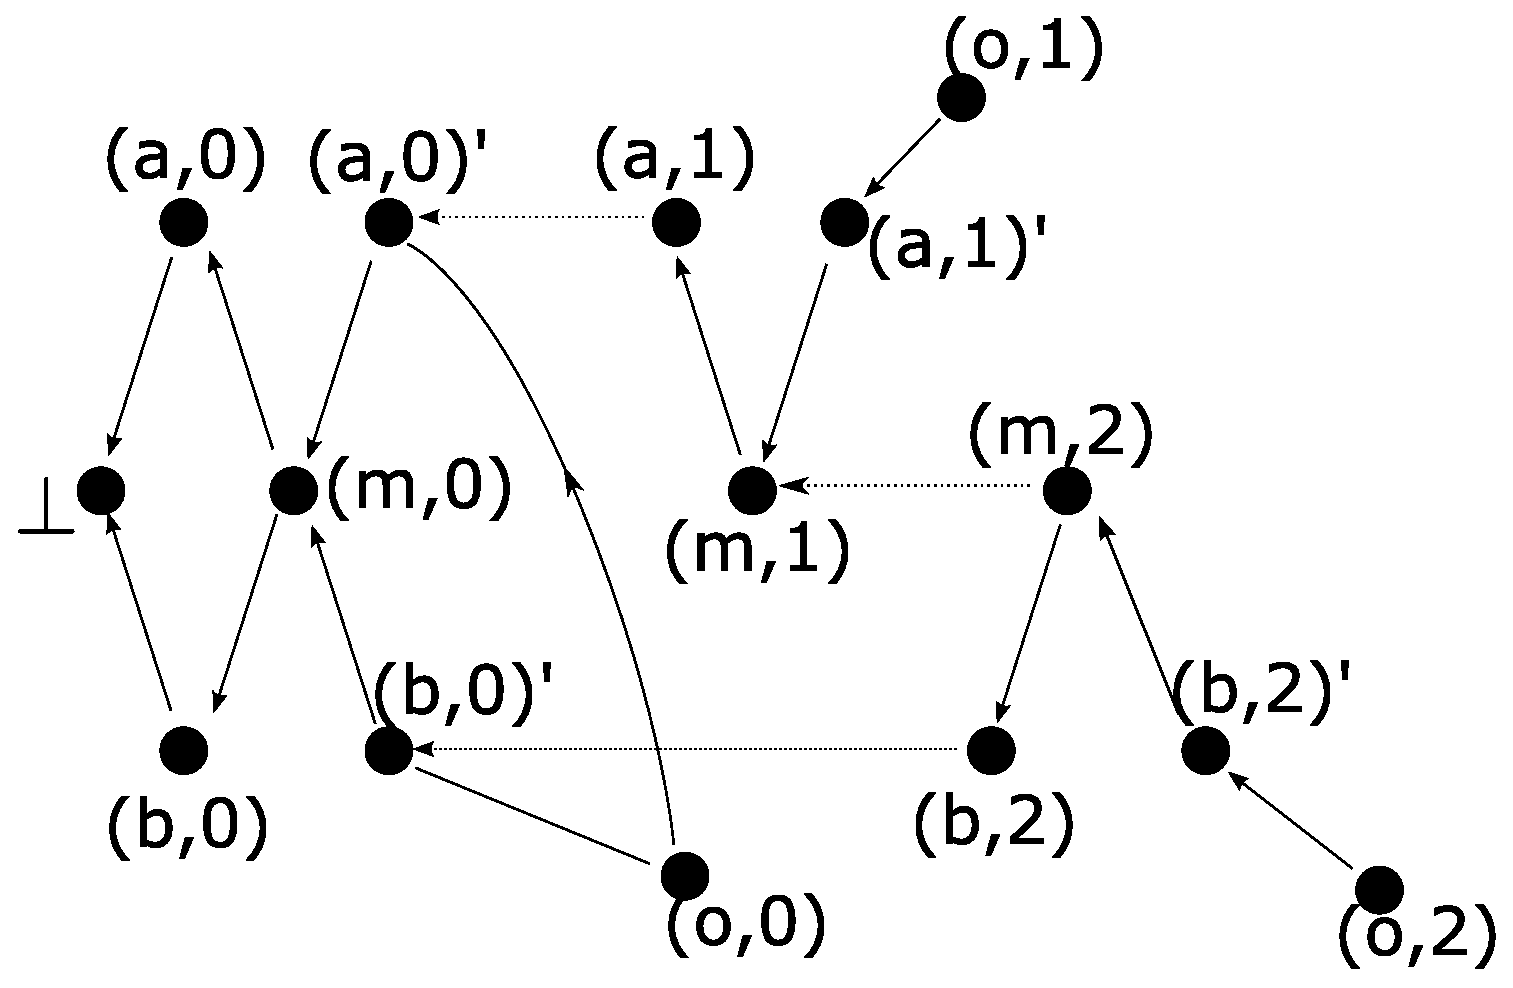
\includegraphics[scale=0.3]{schedulemodel.eps}
   \caption[A model $R(\cdot, \sigma)$.]{A model $R(\cdot, \sigma)$
   induced by the partial schedule $\sigma = \left(\{a,b\}, \{a\}, \{b\}\right)$.
   A solid arrow pointing to $(x,n)$ shows an $f_x$ mapping.  Dotted arrows show $\preceq$ relations.
   We omit implied arrows and the valuation.}
   \label{schedulemodel}
  \end{figure}

  We can state the logical characterisation of waitfree communication.
  \begin{theorem}[Completeness for waitfree communication]
   \label{wf:sc-comp}
   Assume $\varphi\supset \psi$ is a waitfree assertion.
   The relation $\vdash_{SC} \varphi\supset\psi$ holds if the relation $R(\varphi, \sigma),
   (o,n) \models \psi$ holds for any compatible partial schedule $\sigma$ where the state~$(o,n)$
   is the last state of the waitfree model $R(\varphi, \sigma)$.
  \end{theorem}
  To prove completeness, we only use special models called singleton
  models induced by a permutation of processes.

  \begin{definition}
   For a set of processes $P$, we define $\mathsf S(P)$ to be the set of the permutations of $P$.
  \end{definition}

  \begin{definition}
   For $\pi\in \mathsf S(P)$ and $0\le k\le |P|$, we define
   $SC(\pi,k)$ to be the set $\{K_\memory K_a I_a\supset K_\memory K_b I_b\mid b\le a\mbox{ in }\pi_0,\ldots \pi_k\}$.
  \end{definition}

  \begin{lemma}
   \label{perm}
   $\vdashsc \bigvee_{\pi\in \mathsf S(A)} SC(\pi, |P|)$ holds.
  \end{lemma}
  \begin{proof}
   It suffices to use rule (SC) many times.
  \end{proof}

  \begin{definition}
   For a permutation $\pi$ of $P$ and a waitfree protocol description $\varphi$, we
   define a partial schedule $\sigma(\varphi, \pi)$ as
   \[
   \sigma(\varphi, \pi) =
   \overbrace{\pi_0, \cdots, \pi_0}^{count_{\pi_0}(\varphi)},
   \overbrace{\pi_1, \cdots, \pi_1}^{count_{\pi_1}(\varphi)},
   \cdots \cdots
   \cdots,
   \overbrace{\pi_n,\cdots, \pi_n}^{count_{\pi_n}(\varphi)}.
   \]
  \end{definition}

  \begin{definition}
   A singleton model is a model of the form $R(\varphi, \sigma(\varphi,
   \pi))$. We abbreviate this to $R(\varphi, \pi)$.

   For a singleton model and an index $k\in I$, $w_k$ denotes the minimum external
   observer state above all $\pi_j$~states for $j< k$.
  \end{definition}

  \begin{definition}
   For a waitfree protocol description $\varphi = \bigwedge_{a\in A}
   \overbrace{K_a K_\memory K_a \cdots K_a}^{n_a}
   I_a$, we define the restriction \\
   $\varphi\restriction_{p,k} =
   \bigwedge_{a\in A\restriction_{p,k}} \overbrace{K_a K_\memory K_a \cdots K_a}^{n_a} I_a$,
   where $A\restriction_{p,k} = \{a\mid p_j = a \mbox{ for some
   } j<
   k\}$.
  \end{definition}

  \begin{lemma}
   \label{stronger}
   $R(\varphi, \pi), (o,k)\models \psi\Longrightarrow SC(\pi, k)\vdash
   \varphi\restriction_{\pi,k}\supset\psi$.
  \end{lemma}
  Proof to be found in the author's Master's thesis.

  Any models induced by a partial schedule is finite.  For a waitfree assertion $\varphi$,
  it is decidable whether $\vdashsc \varphi$ holds or not.


  \subsection{Decidability of Solvability of Waitfree Task Specification}

  \begin{definition}
   A waitfree task specification $\psi$ is solvable if there is such a
   waitfree protocol description $\varphi$ that the relation
   $R(\varphi,\sigma), (o,n)\models\psi$ holds for any compatible partial
   schedule $\sigma$ where the state $(o,n)$ is the last state of the
   model $R(\varphi,\sigma)$.
  \end{definition}

  \noindent \textbf{Fact.} The set of solvable waitfree task specifications are
  recursively enumerable because the relation $\vdashsc$ is axiomatised.

  \noindent \textbf{Fact.} The set of unsolvable waitfree task
  specifications are recursively enumerable because partial schedule-induced
  models are recursively enumerable.

  \begin{proposition}
   \label{wf-dec}
   It is decidable whether a waitfree task
   specification is solvable or not.
  \end{proposition}
  \begin{proof}
   By the previous two facts.
  \end{proof}

  This does not contradict to the undecidability
  of waitfreely solvable tasks by Gafni and
  Koutsoupias~\cite{gafni1999three}
  because the undecidability proof
  utilises tasks that cannot be expressed by waitfree task specifications.
  They use tasks involving consensus:
  the tasks involving making agreements among processes, where
  whether an output value is allowed or not depends on other processes'
  output values.  Waitfree task specifications cannot describe such tasks.

 \section{Related Work}
 \label{first:related}

 Van Benthem~\cite{van2009information} investigates the connection between
 intuitionistic logic and information dynamics.  He speculates:
 \begin{quotation}
  It might be
  that intuitionistic logic points the way towards a grand synthesis of information analysis
  in the standard model-theoretic style with the dynamic view of logic as embodied
  in proof and games.
 \end{quotation}
 This paper replies his speculation by defining knowledge in terms of BHK-interpretation
 and defining a proof system \iec\,embodying the interpretation.

 Ondrej Majer's
 Epistemic Logic with Relevant Agents~\cite{majer-epistemic}
 is similar to \iec\, in that both logics have epistemic modalities and that both logics are
 not classical.
 However, the logic given in~\cite{majer-epistemic}
 contains only one modality $K$ for knowledge.
 This implicitly assumes that there is a single agent, not multiple agents so that it is
 impossible for their logic to treat communication between multiple agents.

 Many logics have both temporal and epistemic modalities~\cite{sato13study, wozna2005logic}.
 Ewald~\cite{1986} proposes an intuitionistic logic with temporal modality.
 We unify the intuitionistic semantics and temporal semantics so that the logic
 \iec\,lacks temporal modality yet represents some temporal notions.
 Adding a temporal modality like Ewald~\cite{1986} would increase the expressivity of the
 logic, but it would complicate the syntax and semantics.
 We would like to investigate the simple logic \iec\,first
 and then expand \iec\,with
 additional constructs.

 In Kobayashi and Yonezawa's logic~\cite{kobayashi1995asynchronous}, processes
 appear in formulae but time does not appear in formulae
 because time is implicit in the system of logic programming.
 This logic is different from \iec\, in that this logic is based on linear logic and that their
 usage is logic programming.

 Belnap and Harper's ``seeing to it that'' (stit) logical operator
 aims at describing interaction between agents.
 The semantics for the operator involves both agency and temporal notion, which is more
 complicated than the meaning of $K_a$ operator in \iec.
 A fundamental difference of the stit operator and the epistemic operator in \iec\,
 is whether the modalities mention the future or tha past.
 The stit operator mentions the future while the epistemic operator mentions the past.

 Dynamic epistemic logic is a logic that aims at reasoning about communication.
 However the semantics of the logic involves
 instantaneous change of models.
 We argue such instantaneous change of the whole world it is
 not a natural description of asynchronous communication.


 \section{Conclusion}
 \label{conclusion}


 On the logic~\iec, we analysed the concept of sequential consistency and waitfree
 communication.
 The depth of our anlaysis is represented in a deep proof tree (Figure~\ref{hoge}) for a
 property of a relatively simple and small waitfree protol involving two processes.
 Distributed programming over shared memory can be seen as a game involving the scheduler
 and the program.
 Logic can be seen as a game involving the models and the formulae.
 We modelled schedules as a model of logic and programs as formulae.
 Since sequential consistency is a restriction on schedules,
 we modeled sequential consistency as a restriction on models.
 The restriction on the models representing sequential consistency could actually
 axiomatized using an axiom type that is similar to the axiom type for prelinerity defining
 a famous intermediate logic.
 Since waitfreedom is a restriction on programs,
 we modelled waitfree programs as a set of formulae called waitfree protocol description.
 We also modelled specification for waitfree programs as a set of formulae called waitfree
 task specification.
 We used a waitfree assertion, which is
 an implication formula consisting of a waitfree protocol description and a
 waitfree task specification,
 to represent
 an assertion that a waitfree protocol meets a specification.
